\documentclass{minimal}

\usepackage[paperwidth=10.025cm, paperheight=10.025cm, margin=0cm]{geometry}
\setlength{\parindent}{0em}

\usepackage{tikz}

\begin{document}
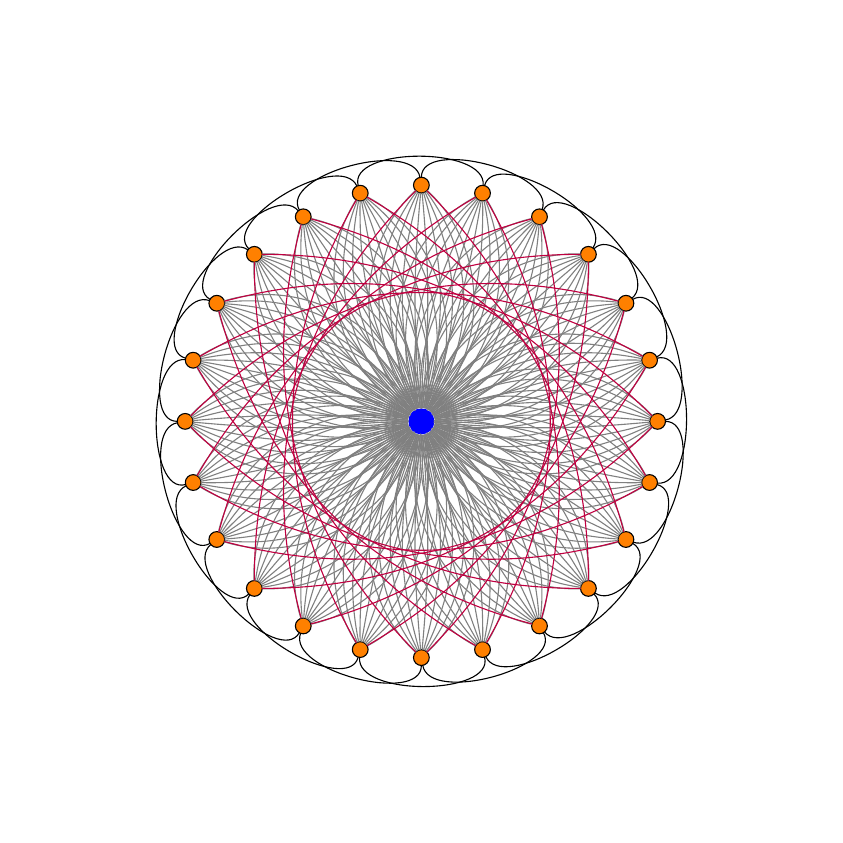
\begin{tikzpicture}[x=1cm, y=1cm, z=1cm]
  \path (-5, -5) rectangle (5, 5);
  %
  \newcommand{\myRadius}{3}
  %
  \node[circle, fill=blue, draw=gray, dotted] at (0, 0) (center) {};
  %
  \newcommand{\numticks}{24}
  \pgfmathsetmacro{\bound}{\numticks - 1}
  \pgfmathsetmacro{\deltaTheta}{360 / \numticks}
  %
  \foreach \i in {0,...,\bound} {
    \pgfmathsetmacro{\myTheta}{\deltaTheta * \i}
    \pgfmathsetmacro{\x}{\myRadius * cos \myTheta}
    \pgfmathsetmacro{\y}{\myRadius * sin \myTheta}
    %
    \draw[fill=orange] (\x, \y) circle (1mm) coordinate (n \i);
    \foreach \j in {-45,-35,...,45}{
      \draw[shorten >=1mm, gray] (center) to[bend left=\j] (n \i);
    }
  }
  %
  % \draw[fill=red] (n 7) circle (1mm);
  %
  \newcommand{\angleOffset}{10}
  \foreach \i in {0,...,\bound} {
    \pgfmathsetmacro{\ii}{Mod(\i + 2, \numticks)}
    \pgfmathsetmacro{\iii}{Mod(\i + 10, \numticks)}
    \pgfmathsetmacro{\thetaOut}{\deltaTheta * \i + \angleOffset}
    \pgfmathsetmacro{\thetaIn}{\deltaTheta * \ii}
    %
    \draw[shorten >=1mm, shorten <=1mm]
      (n \i) to[in=\thetaIn, out=\thetaOut] (n \ii);
    \draw[shorten >=1mm, shorten <=1mm, purple]
      (n \i) to[bend right] (n \iii);
  }
  %\draw (n 1) to[out=10, in=15, looseness=5] (n 2);

\end{tikzpicture}
\end{document}
